% -*- mode: noweb; noweb-default-code-mode: R-mode; -*-
\documentclass[a4paper]{article}

\usepackage{a4wide}
\usepackage{lscape}
\usepackage[margin=.2in]{geometry}

\title{Heritability by Subgroup}
\author{Joe Rodger's BG Team}

\usepackage{Sweave}
\begin{document}
\maketitle


% Here is some text that is rendered almost explictly
Gen2 Link Version: 2011V28.  DV Names: 'HtSt1' and 'HtSt2' in

'F:/Projects/Nls/Links2011/Analysis/Df/2011-12-18/DoubleEntered.csv'.

%This uses DF method 3, where only two coefficients are estimated (Rodgers and Kohler, 2005, BG).
This uses OpenMX, based off the example that David emailed Dec 16, 2011.  The dataset was reduced to single entered.

Implicit ambiguous sibs were assigned R=0.375. Z-Scores are restricted to  +/-10.  All height measures are from 19-25 years of age, standardized by gender (Kelly restandardized early December 2011).  Counts reflect the double entry.
% latex table generated in R 2.14.0 by xtable 1.6-0 package
% Sun Dec 18 18:34:43 2011
\begin{table}[ht]
\begin{center}
\begin{tabular}{lr|rrr|rrr|rrrrr|rrrr}
 Subgroup & $N$ & $h^2$ & $c^2$ & $e^2$ & $\bar{X}$ & $\sigma$ & $\sigma^3$ & $N_{.25}$ & $N_{.375}$ & $N_{.5}$ & $N_{.75}$ & $N_{Mz}$ & $r_{.25}$ & $r_{.375}$ & $r_{.5}$ & $r_{Mz}$ \\ 
 Total & 3458 & 0.81 & 0.00 & 0.19 & -0.02 & 1.00 & -0.04 & 2114 & 0 & 4776 & 0 & 26 & 0.25 &  & 0.39 & 0.95 \\ 
   \hline
FF & 872 & 0.94 & 0.00 & 0.05 & -0.04 & 0.97 & 0.07 & 562 & 0 & 1172 & 0 & 10 & 0.32 &  & 0.45 & 0.95 \\ 
  MF & 1722 & 0.57 & 0.08 & 0.35 & 0.02 & 1.00 & -0.11 & 1062 & 0 & 2382 & 0 & 0 & 0.23 &  & 0.36 &  \\ 
  MM & 864 & 0.81 & 0.00 & 0.19 & -0.08 & 1.00 & -0.03 & 490 & 0 & 1222 & 0 & 16 & 0.20 &  & 0.37 & 0.94 \\ 
   \hline
Hispanic & 871 & 0.28 & 0.26 & 0.46 & -0.39 & 0.93 & 0.11 & 396 & 0 & 1346 & 0 & 0 & 0.33 &  & 0.40 &  \\ 
  Black & 1409 & 0.59 & 0.02 & 0.39 & -0.01 & 1.00 & 0.03 & 1324 & 0 & 1484 & 0 & 10 & 0.18 &  & 0.30 & 0.88 \\ 
  NBNH & 1178 & 0.74 & 0.00 & 0.26 & 0.23 & 0.95 & -0.28 & 394 & 0 & 1946 & 0 & 16 & 0.27 &  & 0.34 & 0.95 \\ 
   \hline
Hisp FF & 204 & 0.02 & 0.45 & 0.53 & -0.43 & 0.89 & 0.15 & 106 & 0 & 302 & 0 & 0 & 0.42 &  & 0.47 &  \\ 
  Hisp MF & 416 & 0.47 & 0.14 & 0.39 & -0.34 & 0.96 & 0.11 & 190 & 0 & 642 & 0 & 0 & 0.27 &  & 0.37 &  \\ 
  Hisp MM & 251 & 0.08 & 0.35 & 0.57 & -0.43 & 0.92 & 0.04 & 100 & 0 & 402 & 0 & 0 & 0.35 &  & 0.40 &  \\ 
   \hline
Black FF & 384 & 0.15 & 0.24 & 0.61 & 0.00 & 0.98 & 0.08 & 376 & 0 & 388 & 0 & 4 & 0.28 &  & 0.31 & 0.80 \\ 
  Black MF & 707 & 0.48 & 0.07 & 0.46 & 0.02 & 1.02 & -0.00 & 664 & 0 & 750 & 0 & 0 & 0.18 &  & 0.31 &  \\ 
  Black MM & 318 & 0.53 & 0.00 & 0.47 & -0.08 & 1.01 & 0.04 & 284 & 0 & 346 & 0 & 6 & 0.07 &  & 0.24 & 0.89 \\ 
   \hline
NBNH FF & 284 & 0.98 & 0.00 & 0.02 & 0.19 & 0.94 & -0.05 & 80 & 0 & 482 & 0 & 6 & 0.20 &  & 0.47 & 0.97 \\ 
  NBNH MF & 599 & 0.32 & 0.15 & 0.53 & 0.26 & 0.95 & -0.41 & 208 & 0 & 990 & 0 & 0 & 0.26 &  & 0.30 &  \\ 
  NBNH MM & 295 & 0.71 & 0.00 & 0.29 & 0.22 & 0.96 & -0.24 & 106 & 0 & 474 & 0 & 10 & 0.32 &  & 0.30 & 0.94 \\ 
  \end{tabular}
\caption{Height Heritability}
\label{tab:two}
\end{center}
\end{table}%\end{landscape}
%%%%%%%%%%%%%%%%%%%%%%%%%%%%%%%%%%%%%%%%%%%%%%%%%%%%%%%%%%%%%%%%%%%%%%
% Get the results for the graphs
%%%%%%%%%%%%%%%%%%%%%%%%%%%%%%%%%%%%%%%%%%%%%%%%%%%%%%%%%%%%%%%%%%%%%%
%Total
 %Default size for remaining graphs
\section{Total Sample}
\begin{figure}[htbp]

\includegraphics{HeritabilitySweave-003}
\end{figure}
Plot Explanation: Each row of graphs isolates a subgroup.  

Each cell in a row isolates a unique value of R; this is displayed in the gray header above each cell. 

Axis and hexbin sizes are constants across all rows.

The orange line is the LS regression for the row (repeated in each cell).

The yellow line is the LS regression for the cell.

The green line is the loess for each cell.  It's bandwidth is not constant across allrows.

The hexbin density color is not constant across rows.

Relevant portions of the table are repeated on each page.
\newpage
\section{By Gender}
% latex table generated in R 2.14.0 by xtable 1.6-0 package
% Sun Dec 18 18:34:48 2011
\begin{table}[ht]
\begin{center}
\begin{tabular}{l|rrr|rrrrr|rrrr}
 Subgroup & $h^2$ & $c^2$ & $e^2$ & $N_{.25}$ & $N_{.375}$ & $N_{.5}$ & $N_{.75}$ & $N_{Mz}$ & $r_{.25}$ & $r_{.375}$ & $r_{.5}$ & $r_{Mz}$ \\ 
 Total & 0.81 & 0.00 & 0.19 & 2114 &   0 & 4776 &   0 &  26 & 0.25 &  & 0.39 & 0.95 \\ 
   \hline
FF & 0.94 & 0.00 & 0.05 & 562 &   0 & 1172 &   0 &  10 & 0.32 &  & 0.45 & 0.95 \\ 
  MF & 0.57 & 0.08 & 0.35 & 1062 &   0 & 2382 &   0 &   0 & 0.23 &  & 0.36 &  \\ 
  MM & 0.81 & 0.00 & 0.19 & 490 &   0 & 1222 &   0 &  16 & 0.20 &  & 0.37 & 0.94 \\ 
  \end{tabular}
\end{center}
\end{table}\begin{figure}[htbp]
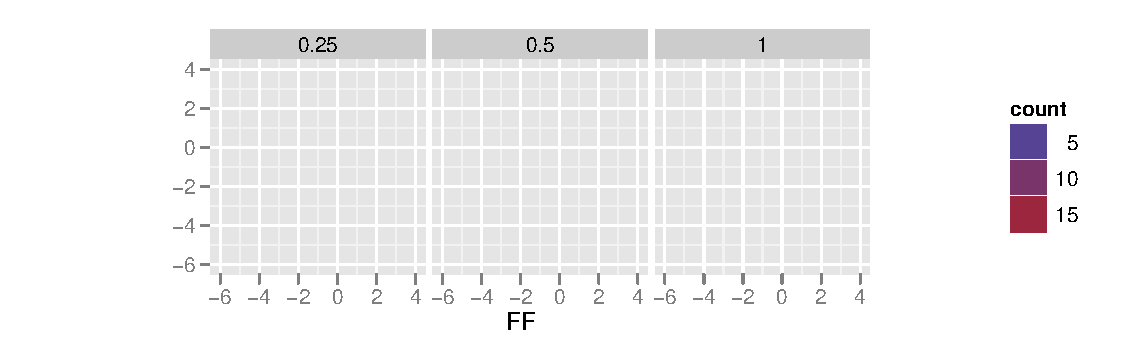
\includegraphics{HeritabilitySweave-005}
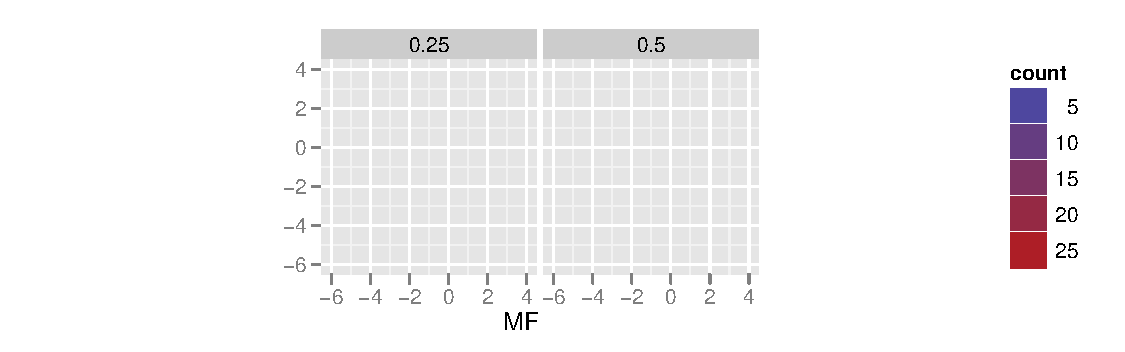
\includegraphics{HeritabilitySweave-006}
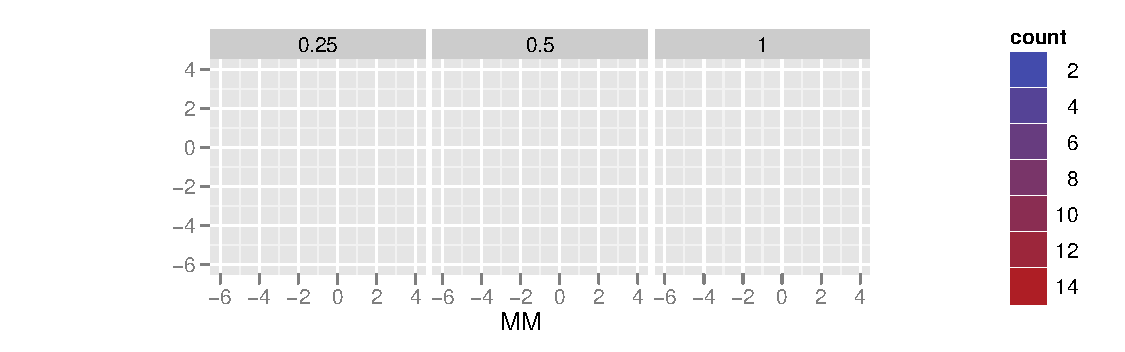
\includegraphics{HeritabilitySweave-007}
\end{figure}

\newpage
\section{By Race}
% latex table generated in R 2.14.0 by xtable 1.6-0 package
% Sun Dec 18 18:34:53 2011
\begin{table}[ht]
\begin{center}
\begin{tabular}{l|rrr|rrrrr|rrrr}
 Subgroup & $h^2$ & $c^2$ & $e^2$ & $N_{.25}$ & $N_{.375}$ & $N_{.5}$ & $N_{.75}$ & $N_{Mz}$ & $r_{.25}$ & $r_{.375}$ & $r_{.5}$ & $r_{Mz}$ \\ 
 Total & 0.81 & 0.00 & 0.19 & 2114 &   0 & 4776 &   0 &  26 & 0.25 &  & 0.39 & 0.95 \\ 
   \hline
Hispanic & 0.28 & 0.26 & 0.46 & 396 &   0 & 1346 &   0 &   0 & 0.33 &  & 0.40 &  \\ 
  Black & 0.59 & 0.02 & 0.39 & 1324 &   0 & 1484 &   0 &  10 & 0.18 &  & 0.30 & 0.88 \\ 
  NBNH & 0.74 & 0.00 & 0.26 & 394 &   0 & 1946 &   0 &  16 & 0.27 &  & 0.34 & 0.95 \\ 
  \end{tabular}
\end{center}
\end{table}\begin{figure}[htbp]
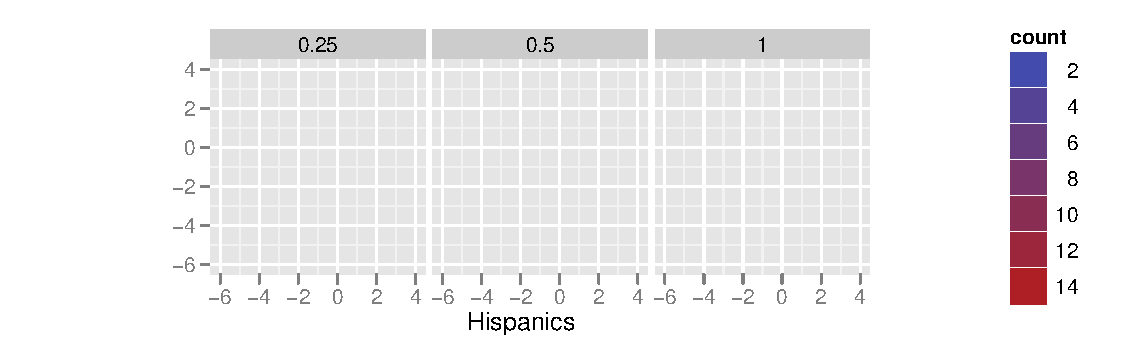
\includegraphics{HeritabilitySweave-009}
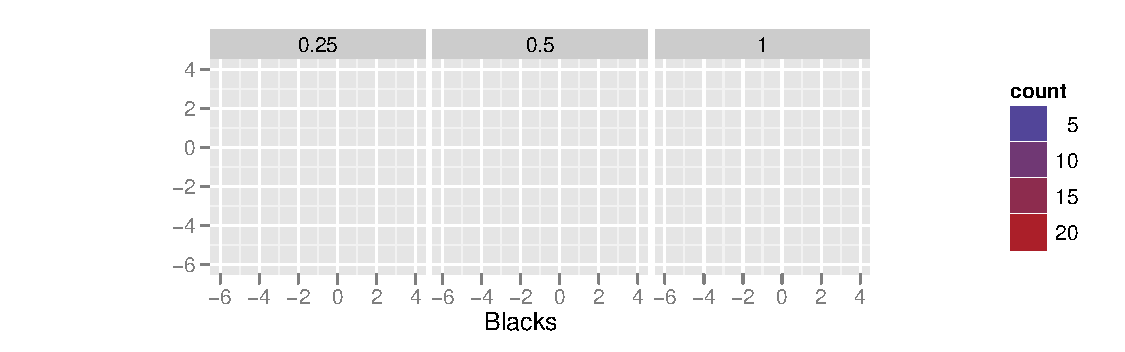
\includegraphics{HeritabilitySweave-010}
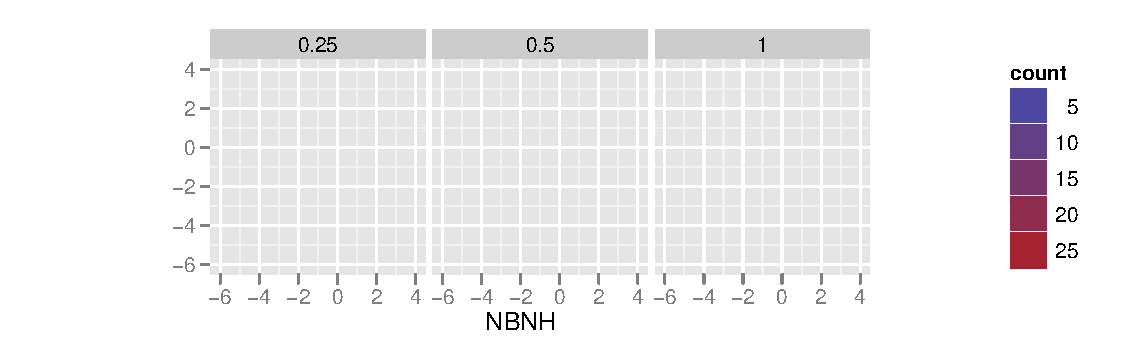
\includegraphics{HeritabilitySweave-011}
\end{figure}
\end{document}
